
\documentclass[calculator,steamtables,refrigeranttables,psychrometricchart,datasheet,solutions,resit]{exam}
%\documentclass[calculator,steamtables,refrigeranttables,psychrometricchart,datasheet,resit]{exam}

% The full list of class options are
% calculator : Allows approved calculator use.
% datasheet : Adds a note that data sheet are attached to the exam.
% handbook : Allows the use of the engineering handbook.
% resit : Adds the resit markings to the paper.
% sample : Adds conspicuous SAMPLE markings to the paper
% solutions : Uses the contents of \solution commands (and \solmarks) to generate a solution file

\usepackage{pdfpages} 
\usepackage{lscape,comment}

\coursecode{EG501J}%%
\coursetitle{Renewable Energy: Solar and Geothermal}%
%\coursecode{EG3539}%
%\coursetitle{Thermodynamics}%

\examtime{00.00--00.00}%
\examdate{00}{05}{2015}%
\examformat{Candidates must attempt \textit{all} questions.}

\newcommand{\frc}{\displaystyle\frac}
\newcommand{\br}[1]{\!\left( #1 \right)}
\newcommand{\abs}[1]{\left| #1 \right|}
\newcommand{\fracd}[2]{\frac{\mathrm{d} #1}{\mathrm{d} #2}}
\newcommand{\fracp}[2]{\frac{\partial #1}{\partial #2}}
\renewcommand{\d}[1]{\mathrm{d} #1 } 
\newcommand{\Ma}{\mathrm{M\!a}} 



\begin{document}

%%%
%%% Question 01 
%%%
\begin{question}
  An engineer decided to use a geothermal source from the yard to keep her Scottish house warm during the winter. The designed heat pump extracts water from the well at 15$^{\circ}$C and discharges at 8$^{\circ}$C. As working fluid, she decided to use propane $\left(\text{n-C}_{3}\right)$ -- see Figure below, that will transfer heat into a constant stream of cold air $\left(\dot{m}_{\text{air}}=\text{2 kg.s}^{-1}\right)$ at 12$^{\circ}$. 
\vspace{-1cm}
\begin{center}
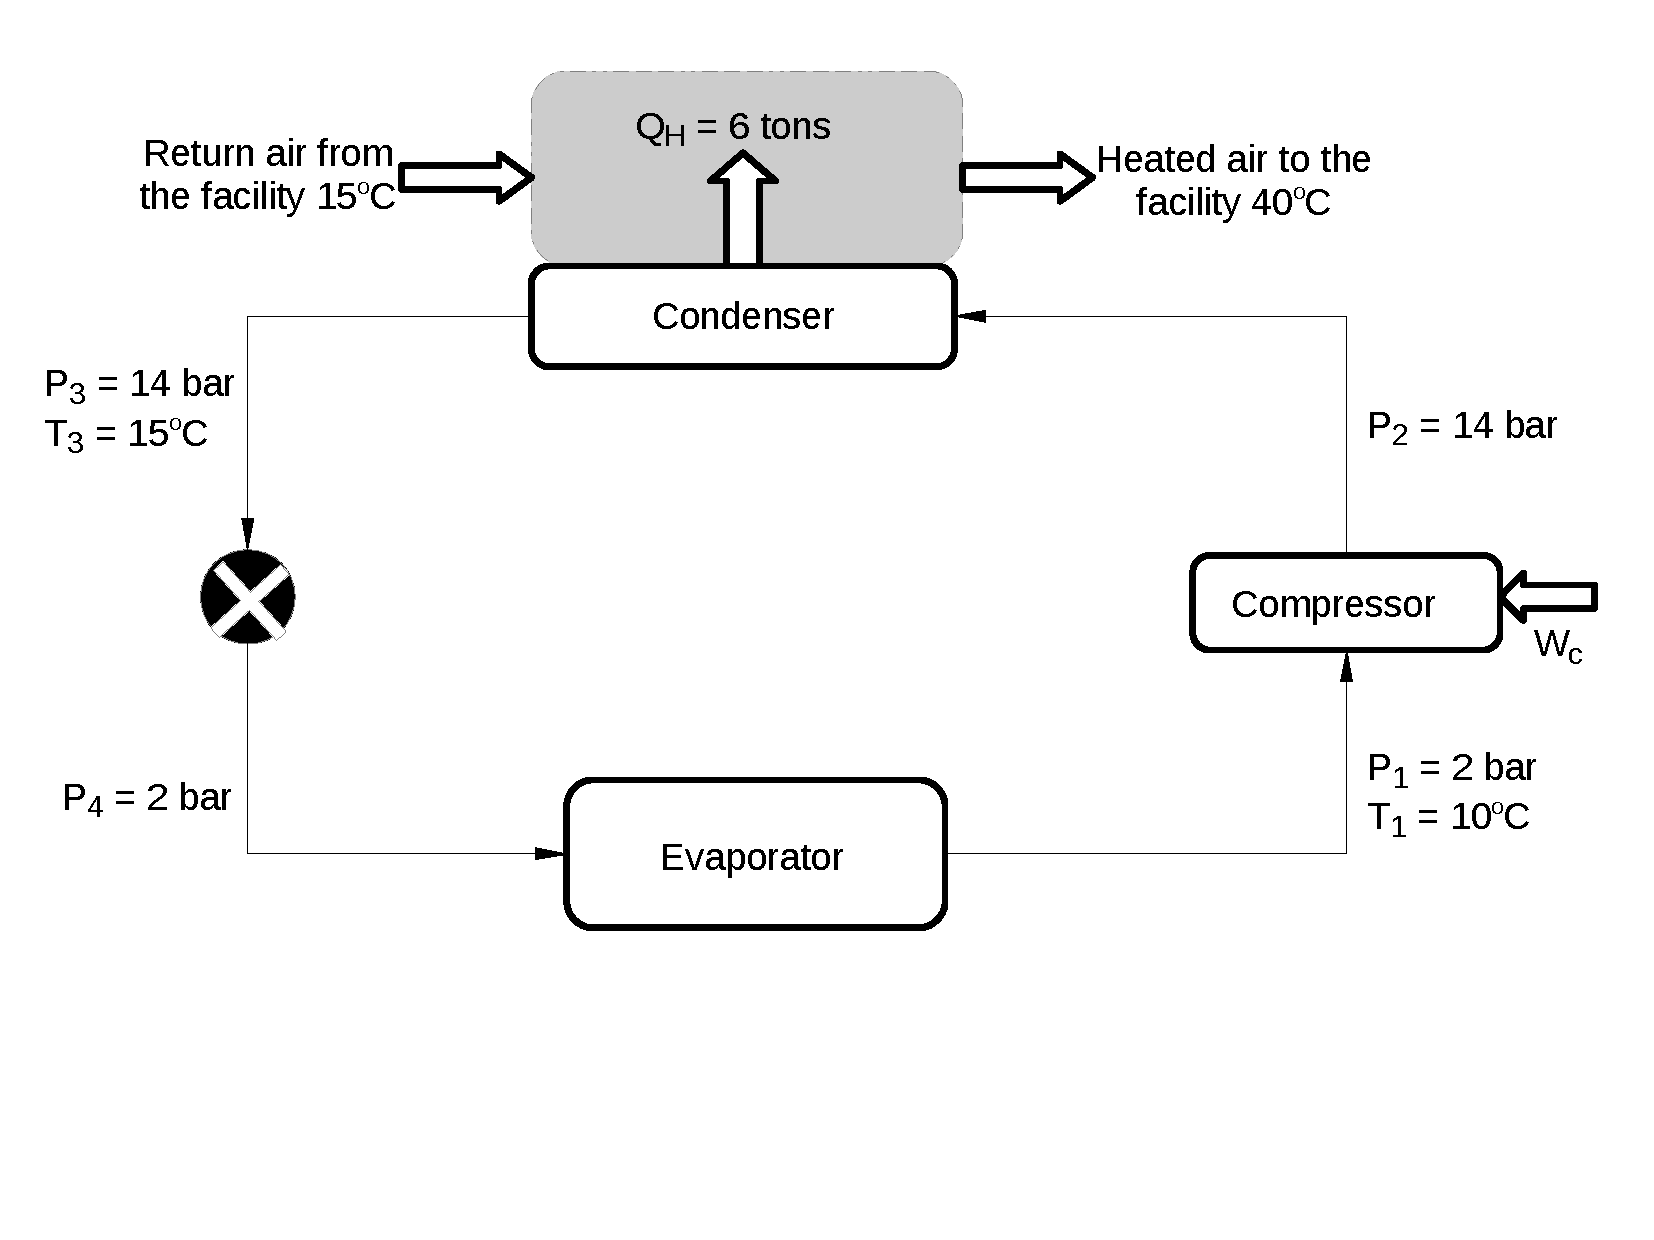
\includegraphics[width=9.0cm,height=7.0cm]{./Pics/Overview_Refrig42}
\end{center}
\begin{enumerate}[(a)]
%
\item Calculate enthalpies and entropies of streams 1-4.~\marks{8}
\solution{\begin{description}
%
\item[Stage 1:] At P$_{1}$ = 3 bar and T$_{1}$ = 0$^{\circ}$C $\Longrightarrow$ T$_{\text{sat}}$ = -14.16$^{\circ}$C $<$ T$_{1}$, thus n-C$_{3}$ is at superheated state (SHF). Thus, from SHF table, {\bf H$_{1}$=477.1 kJ.kg$^{-1}$}~\solmarks{1/8} and {\bf S$_{1}$ = 1.851 kJ.(kg.K)$^{-1}$}.~\solmarks{1/8} 
%
\item[Stage 2:] At P$_{2}$ = 7 bar and T$_{2}$ = 40$^{\circ}$C $\Longrightarrow$ T$_{\text{sat}}$ = 13.41$^{\circ}$C $<$ T$_{2}$, thus n-C$_{3}$ is at superheated state (SHF). Thus, from SHF table, {\bf H$_{2}$=534.8 kJ.kg$^{-1}$}~\solmarks{1/8} and {\bf S$_{2}$ = 1.901 kJ.(kg.K)$^{-1}$}.~\solmarks{1/8} 
%
\item[Stage 3:] At P$_{3}$ = 7 bar and T$_{3}$ = 10$^{\circ}$C $\Longrightarrow$ T$_{\text{sat}}$ = 13.41$^{\circ}$C $>$ T$_{2}$, thus n-C$_{3}$ is a sub-cooled fluid. Thus, from saturated table, {\bf H$_{3}$=196.7 kJ.kg$^{-1}$}~\solmarks{1/8} and {\bf S$_{2}$ = 0.716 kJ.(kg.K)$^{-1}$}.~\solmarks{1/8} 
%
\item[Stage 4:] At P$_{4}$ = 3 bar $\Longrightarrow$ Isenthalpic expansion, thus {\bf H$_{4}$} = H$_{3}$ {\bf = 196.7 kJ.kg$^{-1}$}~\solmarks{1/8}. In order to calculate the entropy, we first need to calculate the quality of the fluid,
\begin{displaymath}
x_{4} = \frc{H_{4} -  H_{f}}{H_{g} - H_{f}} = \frc{196.7-60.3}{453.6 - 60.3} = 0.3468
\end{displaymath} 
\begin{displaymath}
x_{4} = 0.3468 = \frc{S_{4}-S_{f}}{S_{g}-S_{f}} = \frc{S_{4}-0.244}{1.762-0.244} \Longrightarrow {\bf S_{4} = 0.7704 \frc{kJ}{kg.K}}
\end{displaymath}\solmarks{1/8}
%
\end{description}
}
%
\item For a mass flow rate of n-C$_{3}$ $\left(\dot{m}_{\text{C3}}\right)$ of 10$^{-2}$ kg.s$^{-1}$, calculate the required water flow rate. The heat capacity $\left(\text{C}_{p}\right)$ of water is 4.1813 kJ.(kg.K)$^{-1}$.~\marks{2}
%
\solution{
The heat exchange in the evaporator can be expressed as:
\begin{eqnarray}
 -\dot{m}_{C3}\left(H_{1}-H_{4}\right) = \dot{m}_{w}\left(H_{w}^{out} - H_{w}^{in}\right) = \dot{m}_{w} C_{p,w} \left(T_{w}^{in}-T_{w}^{out}\right) \nonumber \\
 -10^{-2}\left(477.1-196.7\right) = \dot{m}_{w} \times 4.1813 \times\left(8 - 15\right) \Longrightarrow {\bf \dot{m}_{w} = 0.0958 \frc{kg}{s}} \nonumber 
\end{eqnarray}~\solmarks{2/2}
} 
%
\item Assuming that all heat extracted in the condenser is transferred to the air stream $\left(\dot{m}_{\text{air}}=\text{2 kg.s}^{-1}\right)$, calculate the temperature of this heated stream $\left(\text{T}_{\text{out}}^{\text{air}}\right)$.~\marks{5}
%
\solution{
The heat exchange in the condenser is expressed as
\begin{displaymath}
{\bf Q_{H}} = \dot{m}_{C3}\left(H_{2}-H_{3}\right) {\bf = 32.39 \frc{kJ}{kg}}
\end{displaymath}~\solmarks{2/5}
Assuming that there is no heat loss,
\begin{displaymath}
Q_{4} = 32.39 = \dot{m}_{\text{air}} C_{p,air}\left(T^{\text{air}}_{\text{out}}-T^{\text{air}}_{\text{in}}\right) = 2 \times 1.004\times\left(T^{\text{air}}_{\text{out}} - 12\right) \Longrightarrow {\bf T^{\text{air}}_{\text{out}} = 28.13^{\circ}C}
\end{displaymath}~\solmarks{3/5}
}
%
\item Nearby the engineer's house, a geothermal reservoir was mapped and the following data was gathered, 
\begin{center}
\begin{tabular}{||c | c | c | c| c | c| c ||}
\hline\hline
{\bf Temperature $\left(^{o}C\right)$} & 25 & 40 & 63 & 100 & 155 & 245 \\
{\bf Depth (m)}                        & 0 & 200 & 400 & 600 & 800 & 1000 \\
\hline\hline
\end{tabular}
\end{center}
\begin{enumerate}[(i)]
\item Calculate the temperature gradient of this reservoir.~\marks{2}
%
\solution{
\begin{displaymath}
{\bf \nabla T} = \frc{\partial T}{\partial z} =  \frc{T_{n} - T_{1}}{z_{n} - z_{1}} = \frc{245-25}{1000-0} = {\bf 0.22\frc{^{\circ}C}{m}} 
\end{displaymath}~\solmarks{2/2}
}
%
\item Binary cycle geothermal power plants operate at a temperature range between 107 and 182$^{\circ}$C. Assuming there is no heat loss in the production well, what is the ideal depth for a source of brine of 143$^{\circ}$C.~\marks{3}
%
\solution{The depth can be obtained via linear interpolation at 100$\leq$T$\leq$155$^{\circ}$C. At 143$^{\circ}$C the depth is {\bf 756.36 m}~\solmarks{3/3}
}
%
\item Describe how binary cycle geothermal power plants operate.~\marks{5} 
%
\solution{\begin{itemize}
\item Binary cycle geothermal power plants are often operated between 107 $\leq$ T $\leq$ 182$^{\circ}$C;\solmarks{1/5}
\item The produced hot brine vaporises the working fluid and is isentropically expanded in the turbine;\solmarks{2/5}
\item Working fluids often used in geothermal plants are organic chemical species with low boiling temperature.~\solmarks{2/5}
\end{itemize}
}
%
\end{enumerate}
%
\end{enumerate}

\end{question}


To solve this problem, you should assume that the saturated liquid streams are incompressible, and therefore $dH = VdP$ (where $H$, $V$ and $P$ are enthalpy, volume and pressure, respectively). Quality of the vapour is expressed as
\begin{displaymath}
x_{j} = \frc{\Psi_{j}-\Psi_{f}}{\Psi_{g}-\Psi_{f}}\;\;\;\text{with }\Psi=\left\{H,S\right\}
\end{displaymath}
where $S$ is the entropy.



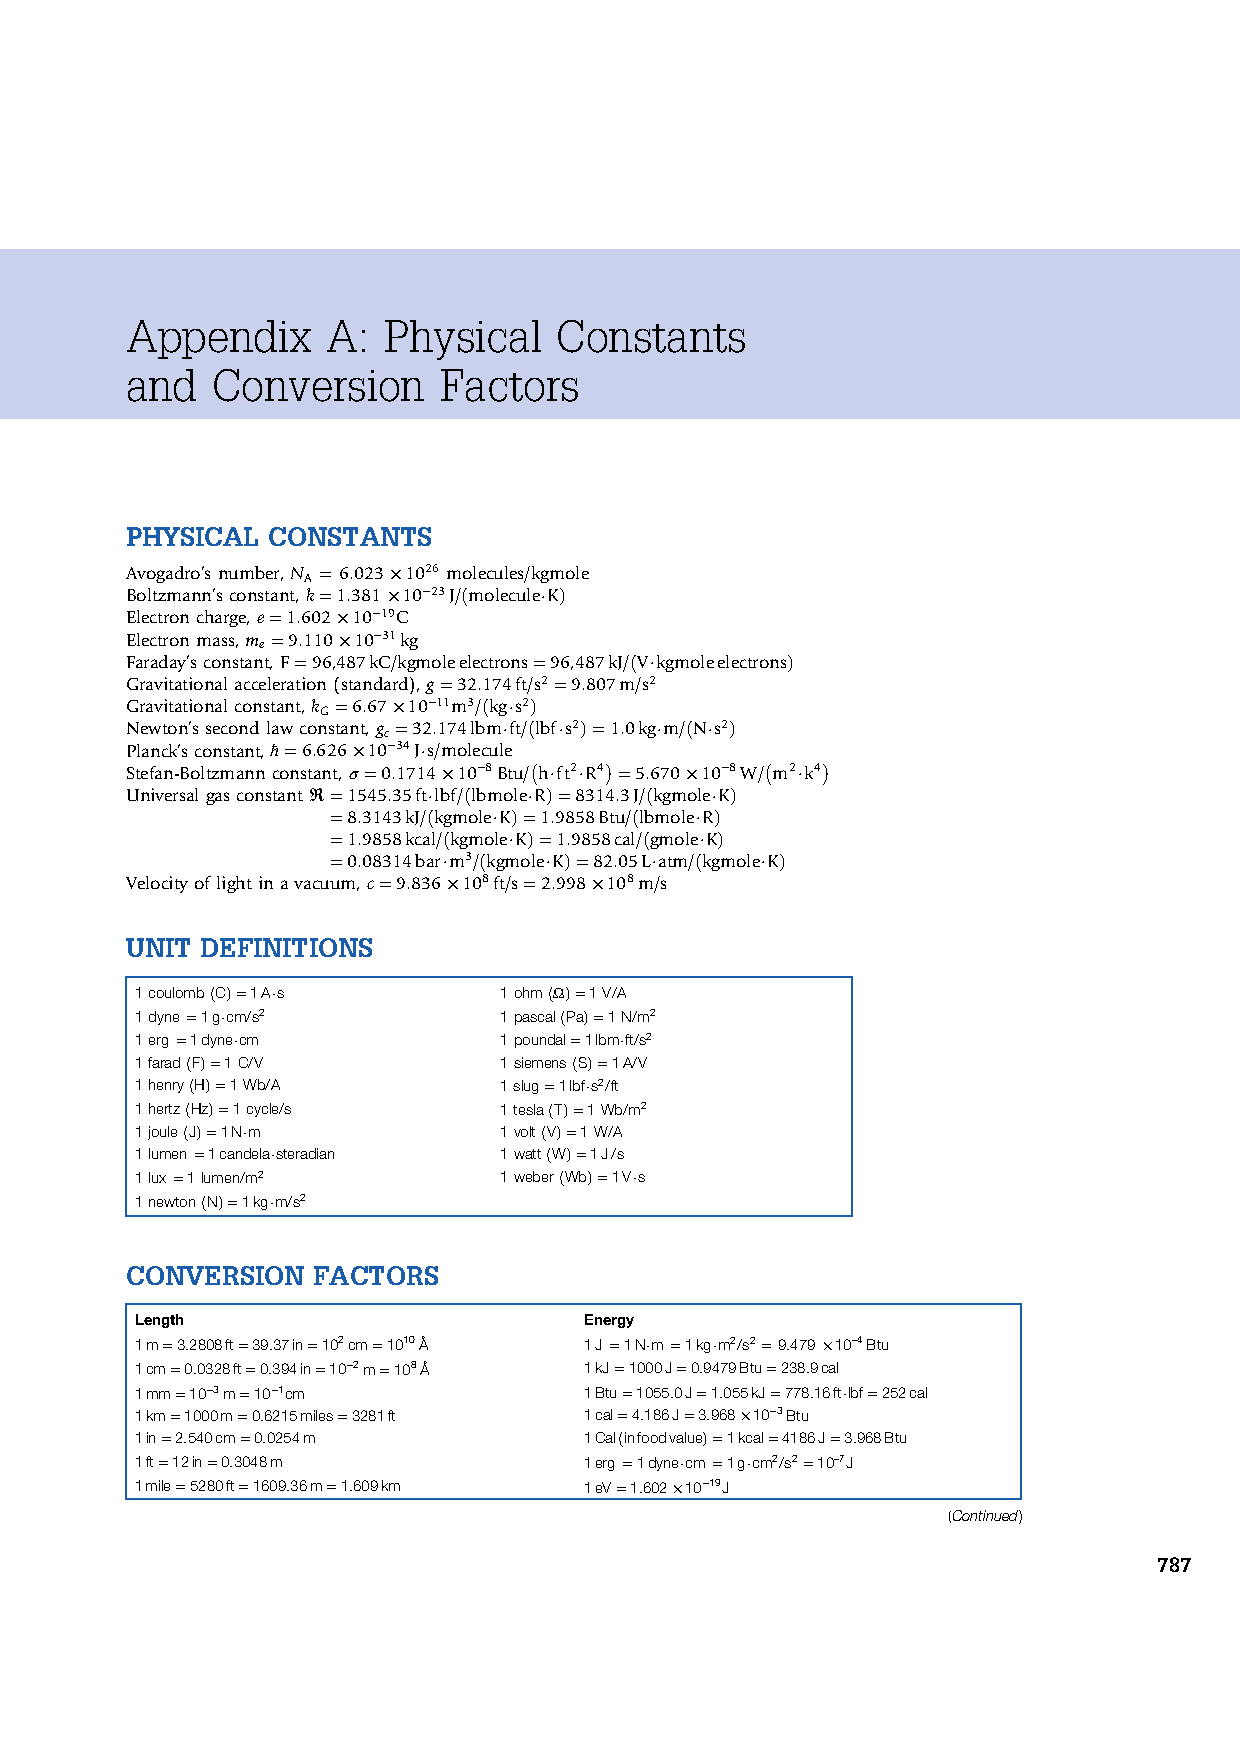
\includepdf[pages={1-6}]{./Pics/nC3_UnitConv}

\clearpage
\end{document}
